
\section{Atividade 6}

\subsection{Introdução ao Modelo com Controlador PID}
Os controladores PID são amplamente reconhecidos por sua eficácia e flexibilidade, combinando três elementos distintos para obter um desempenho superior: proporcional, integral e derivativo. Ao contrário dos controladores proporcionais, que ajustam a resposta do sistema de maneira direta ao erro atual, os controladores PID aproveitam três abordagens diferentes, cada uma desempenhando uma função específica.

O componente proporcional funciona de modo semelhante ao controlador proporcional simples, ajustando a saída do sistema em relação direta ao erro, com o objetivo de reduzir a diferença entre o valor medido e o valor desejado. No entanto, quando o componente proporcional sozinho não consegue corrigir totalmente o erro acumulado, entra em ação o componente integral, que soma e integra o erro ao longo do tempo para eliminá-lo.

Além disso, o componente derivativo desempenha um papel crucial ao prever mudanças no erro, ajudando a evitar que essas variações causem impactos negativos na saída do sistema. Com a integração desses três elementos, os controladores PID conseguem oferecer um controle mais preciso e estável, ajustando continuamente a saída para manter o sistema no estado desejado.
A fórmula padrão de um controlador PID pode ser representada pela equação \ref{eq:pid}:
\begin{equation}
    u(t) = K_p e(t) + K_i \int_{0}^{t} e(T) dT + K_d \frac{d e(t)}{dt}
    \label{eq:pid}
\end{equation}

O método de Ziegler-Nichols, desenvolvido por John G. Ziegler e Nathaniel B. Nichols, é uma técnica consolidada para a sintonia de controladores PID. Este método é particularmente útil porque simplifica a configuração dos controladores ao fornecer fórmulas práticas para calcular os ganhos \( K_p \), \( K_i \), e \( K_d \) com base na resposta do sistema a uma entrada de teste. Esses parâmetros são ajustados para otimizar a resposta do sistema em termos de tempo de subida, sobreposição e tempo de assentamento.

Os valores dos ganhos são estabelecidos de acordo com a estabilidade observada do sistema e são tipicamente calculados a partir do ganho crítico \( K_c \) e do período crítico \( P_c \), que são obtidos através de testes de malha aberta. A Tabela \ref{tab:ziegler-nichols} resume os valores recomendados para cada tipo de ganho:

\begin{table}[h]
    \centering
    \begin{tabular}{ccc}
        \hline
        \( K_p \)            & \( K_i \)                      & \( K_d \)              \\
        \hline
        \( 0,6 \times K_c \) & \( \frac{2}{P_c} \) & \( 0,125 \times P_c \) \\
        \hline
    \end{tabular}
    \caption{Valores dos ganhos segundo o método de Ziegler-Nichols}
    \label{tab:ziegler-nichols}
\end{table}

% ===============================================================
% Letra A Validado ==============================================
\subsection{Controlador PID}

Com base nas análises conduzidas na Atividade 4, foi estabelecido um valor limite para o ganho crítico, \( K_c \), de 14.93. Este parâmetro é crucial para o ajuste dos parâmetros do controlador PID utilizando o método de Ziegler-Nichols. Semelhante ao procedimento adotado na Atividade 5, simulou-se o comportamento do sistema com um sinal de entrada em forma de degrau, cuja amplitude é definida como \( A = \frac{m}{4} \). Considerando que \( m = 10 \), a amplitude do degrau é \( A = 2.5 \). Este cenário permitiu a observação direta das respostas do sistema sob o efeito do ganho crítico.

\begin{figure}[H]
    \centering
    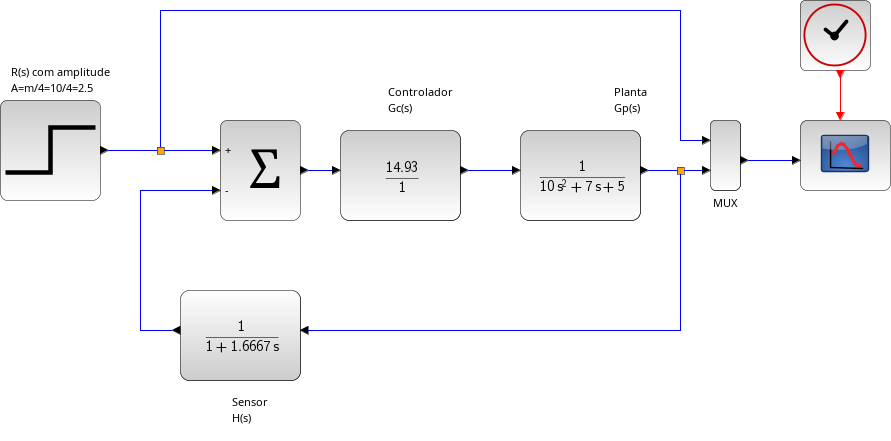
\includegraphics[width=0.7\textwidth]{atividades/6-atividade/assets/a/diagrama-ganho-critico-sistema-instavel.png}
    \caption{Diagrama mostrando o sistema no ponto crítico com \( K_c = 14.93 \)}
    \label{fig:diagrama-ponto-critico}
\end{figure}

A simulação realizada no ganho crítico, \( K_c = 14.93 \), demonstra que o sistema atinge uma condição de oscilação não amortecida, o que é indicativo de uma fronteira entre a estabilidade e a instabilidade. Essa observação é fundamental, pois o ponto de oscilação não amortecida é usado pelo método de Ziegler-Nichols para calibrar os controladores PID, visando uma resposta rápida e minimamente oscilatória em regime permanente.

\begin{figure}[H]
    \centering
    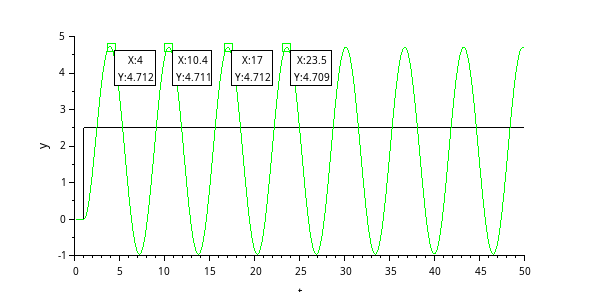
\includegraphics[width=0.7\textwidth]{atividades/6-atividade/assets/a/ganho-critico-sistema-instavel.png}
    \caption{Resposta do sistema com o controlador PID ajustado para \( K_c = 14.93 \)}
    \label{fig:ganho-critico-sistema-instavel}
\end{figure}


Como observado no gráfico de resposta temporal, o sistema exibe oscilações contínuas com uma amplitude aproximadamente constante, confirmando a caracterização do ganho crítico. Esta condição é explorada para determinar o período crítico \( P_c \), calculado pela medição do intervalo entre picos consecutivos. O valor de \( P_c \) é crucial para definir os parâmetros do controlador PID, pois influencia diretamente a dinâmica de correção implementada pelo controlador.

Os dados obtidos deste experimento são essenciais para a calibração dos parâmetros do controlador PID. Ajustar o controlador para operar próximo do ponto crítico, mas com garantias de estabilidade, permite aproveitar a máxima capacidade de resposta do sistema sem comprometer sua segurança operacional. Esta abordagem visa melhorar tanto a eficiência quanto a estabilidade do sistema, tornando o controle mais robusto frente a variações nas condições operacionais.

\subsubsection{Determinação do Período Crítico}
O período crítico \( P_c \) foi determinado a partir da análise do gráfico de resposta em regime oscilatório no ganho crítico. Identificamos os picos consecutivos e medimos o tempo entre eles para calcular o \( P_c \). A partir dos pontos identificados no gráfico, com os tempos \( t_1 = 9.98 \, \text{s} \) e \( t_2 = 16.894 \, \text{s} \), o período crítico foi calculado como:
\[
    P_c = t_2 - t_1 = 16.894 - 9.98 = 6.914 \, \text{s}
\]
Este valor é importante para o ajuste subsequente dos parâmetros do controlador PID utilizando o método de Ziegler-Nichols.


\subsubsection{Determinação dos Parâmetros do Controlador PID}
Após identificarmos o ganho crítico \( K_c = 14.93 \) através de análises detalhadas, empregamos o método de Ziegler-Nichols para ajustar os parâmetros do controlador PID. Este método é eficaz para sintonizar controladores em sistemas onde a resposta precisa ser otimizada em termos de estabilidade e rapidez.

\subsubsection{Cálculo dos Parâmetros do Controlador PID}
O método de Ziegler-Nichols, conhecido por sua eficiência na configuração inicial de controladores PID, utiliza o ganho crítico \( K_c \) e o período crítico \( P_c \) para estabelecer os parâmetros de controle, ajustando assim a resposta do sistema.

\begin{itemize}
    \item \textbf{Ganho Proporcional} \( K_p \):
          \[
              K_p = 0.6 \times K_c = 0.6 \times 14.93 = 8.958
          \]
    \item \textbf{Ganho Integral} \( K_i \):
          \[
              K_i = \frac{2}{P_c} = \frac{2}{6.914} \approx 0.289
          \]
    \item \textbf{Ganho Derivativo} \( K_d \):
          \[
              K_d = 0.125 \times P_c = 0.125 \times 6.914 = 0.864
          \]
\end{itemize}

\subsubsection{Implementação e Validação dos Parâmetros}
Os parâmetros \( K_p = 8.958 \), \( K_i = 0.289 \), e \( K_d = 0.864 \) são implementados no controlador PID no ambiente de simulação Scilab. Esses valores são projetados para ajustar o sistema a fim de responder de forma ideal em diversas condições operacionais, melhorando tanto a estabilidade quanto a precisão do sistema.

A eficácia desses parâmetros será validada por meio de simulações adicionais, que irão confirmar se eles conseguem manter o desempenho desejado do sistema, assegurando que o controle PID seja eficiente e eficaz.

\begin{figure}[H]
    \centering
    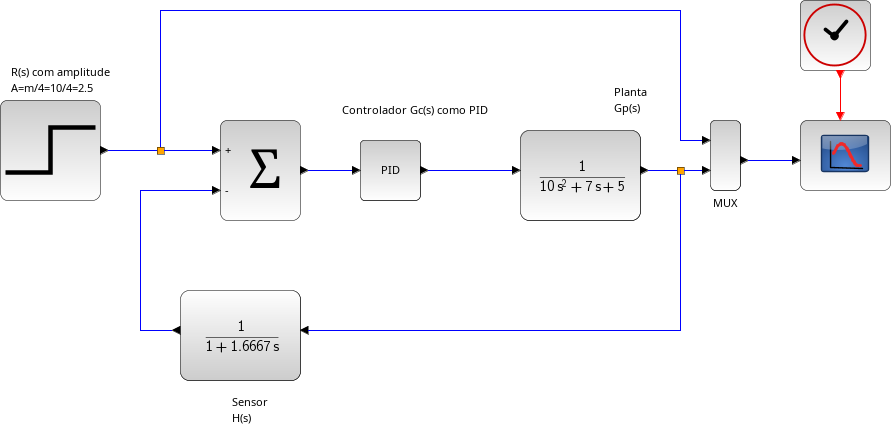
\includegraphics[width=0.8\textwidth]{atividades/6-atividade/assets/a/diagrama-pid.png}
    \caption{Resposta do sistema com os parâmetros do PID ajustados.}
    \label{fig:diagrama-pid}
\end{figure}

\begin{figure}[H]
    \centering
    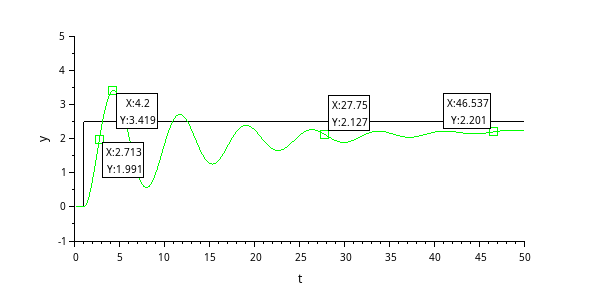
\includegraphics[width=0.8\textwidth]{atividades/6-atividade/assets/a/pid.png}
    \caption{Resposta do sistema com os parâmetros do PID ajustados.}
    \label{fig:resposta-pid}
\end{figure}

Após a validação inicial, pode ser necessário um refinamento manual dos parâmetros para otimizar ainda mais a resposta do sistema. Este processo de ajuste fino baseia-se na análise detalhada das respostas obtidas e na experiência prática, permitindo uma sintonia mais precisa que se adapta adequadamente às especificidades do sistema e às variações nas condições operacionais. Este ajuste é crucial para alcançar o melhor equilíbrio entre estabilidade e rapidez na resposta do controlador PID.

Subsequentemente, novas simulações serão realizadas para validar a eficácia dos parâmetros ajustados. Esta etapa é fundamental para verificar se os ajustes refinados mantêm a saída do sistema próxima ao valor desejado sob uma gama mais ampla de condições operacionais, garantindo a eficácia e a eficiência do controle.

% ===============================================================
% Letra B Validado ==============================================
\subsection{Análise de Resposta com Controlador Proporcional e PID Ajustado}

Esta seção compara a resposta do sistema utilizando um controlador proporcional e um controlador PID ajustado, especificamente configurados com os parâmetros \( K_p = 8.958 \), \( K_i = 0.310 \), e \( K_d = 0.805 \). A análise foca na eficácia de cada controlador em atingir e manter o valor de referência desejado, sob uma amplitude de degrau de \( A = 2.5 \). Este estudo visa elucidar as vantagens e limitações de cada abordagem de controle em termos de resposta dinâmica e estabilidade.

\begin{figure}[H]
    \centering
    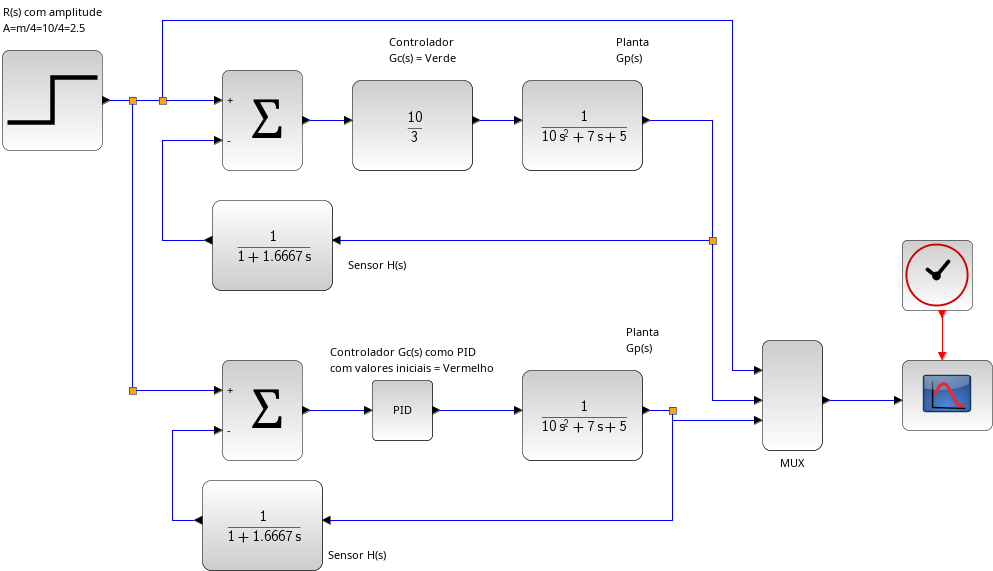
\includegraphics[width=0.8\textwidth]{atividades/6-atividade/assets/b/diagrama-comparacao-proporcional-pid.png}
    \caption{Diagrama ilustrativo do sistema de controle comparando a resposta com controlador proporcional e PID ajustado.}
    \label{fig:diagrama-comparacao-proporcional-pid}
\end{figure}

\begin{figure}[H]
    \centering
    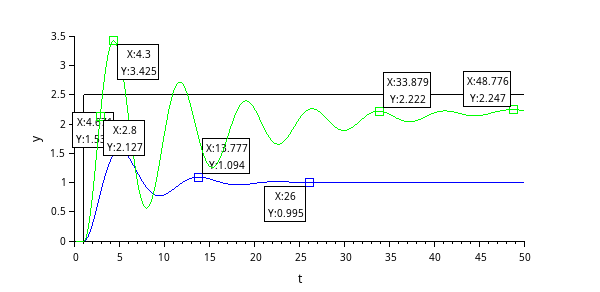
\includegraphics[width=0.8\textwidth]{atividades/6-atividade/assets/b/comparacao-proporcional-pid.png}
    \caption{Resposta temporal do sistema com controlador proporcional e PID ajustado.}
    \label{fig:comparacao-proporcional-pid}
\end{figure}

\subsubsection{Controlador Proporcional (Cor Azul)}
\textbf{Comportamento:}
O controlador proporcional oferece uma resposta imediata, característica desejada em muitas aplicações industriais por sua simplicidade e eficácia em sistemas menos complexos. No entanto, como evidenciado na Figura \ref{fig:comparacao-proporcional-pid}, ele falha em eliminar o erro de estado estacionário, estabilizando abaixo do valor de referência desejado.

\textbf{Estado Estacionário:}
A incapacidade de ajustar o erro estacionário torna o controlador proporcional menos adequado para aplicações que demandam precisão contínua e ajuste fino, pois não pode corrigir desvios permanentes sem intervenção externa.

\subsubsection{Controlador PID Ajustado (Cor Verde)}
\textbf{Comportamento:}
A configuração ajustada do PID demonstra superioridade em alcançar e manter o valor desejado rapidamente, com uma oscilação inicial (overshoot) significativamente reduzida e rápida estabilização, como ilustrado na Figura \ref{fig:comparacao-proporcional-pid}. Essa resposta é crucial em processos que não podem tolerar grandes desvios temporários ou onde o controle preciso é crítico.

\textbf{Estado Estacionário:}
O controlador PID, ajustado com parâmetros otimizados, mantém o valor de referência com alta precisão, ilustrando a importância da ação integral em corrigir erros acumulados e a ação derivativa em antecipar e mitigar futuras variações, resultando em uma resposta estável e precisa.

\subsubsection{Conclusão}
A análise comparativa entre o controlador proporcional e o PID ajustado destaca a simplicidade e a resposta imediata do primeiro, ideal para aplicações menos críticas, contra a precisão e a estabilidade superior do segundo. Com parâmetros ajustados (\(K_p = 8.958\), \(K_i = 0.310462589\), \(K_d = 0.80525\)), o controlador PID se adapta melhor às necessidades de aplicações que exigem controle dinâmico e alta fidelidade.

No entanto, é crucial reconhecer que os ajustes nos parâmetros \(K_p\), \(K_i\), e \(K_d\) do PID não são sem riscos e devem ser continuamente revisados. Alterações imprudentes em \(K_p\) podem levar a overshoots excessivos e instabilidade, enquanto \(K_i\) elevado pode causar oscilações indesejadas e resposta lenta, afetando negativamente a eficácia do sistema. Ajustes em \(K_d\) também requerem cautela, pois, embora possam melhorar a estabilidade, podem resultar em uma resposta demasiadamente amortecida.

Portanto, é recomendado que os ajustes nos parâmetros do PID sejam feitos com base em testes rigorosos e análise cuidadosa. A busca por um equilíbrio ótimo entre rapidez de resposta, estabilidade e precisão deve ser uma prática regular, adaptando o controlador às variações nas condições operacionais e às exigências específicas de cada aplicação. Esse processo contínuo de otimização ajuda a assegurar a performance aprimorada e a segurança do sistema controlado.


% ===============================================================
% Letra C Validado ==============================================
\subsection{Teste de Ajuste de Parâmetros do \( K_p \) do Controlador PID}

\subsubsection{Contextualização e Análise do Ajuste de \( K_p \)}
Para otimizar o desempenho do controlador PID, realizamos uma série de simulações alterando o valor de \( K_p \) para entender seu impacto na dinâmica do sistema. O objetivo foi encontrar um equilíbrio ideal entre a resposta rápida e a estabilidade do sistema, testando \( K_p \) em 80\% e 150\% do valor inicial de 8.958, além do próprio valor inicial.

\begin{figure}[H]
    \centering
    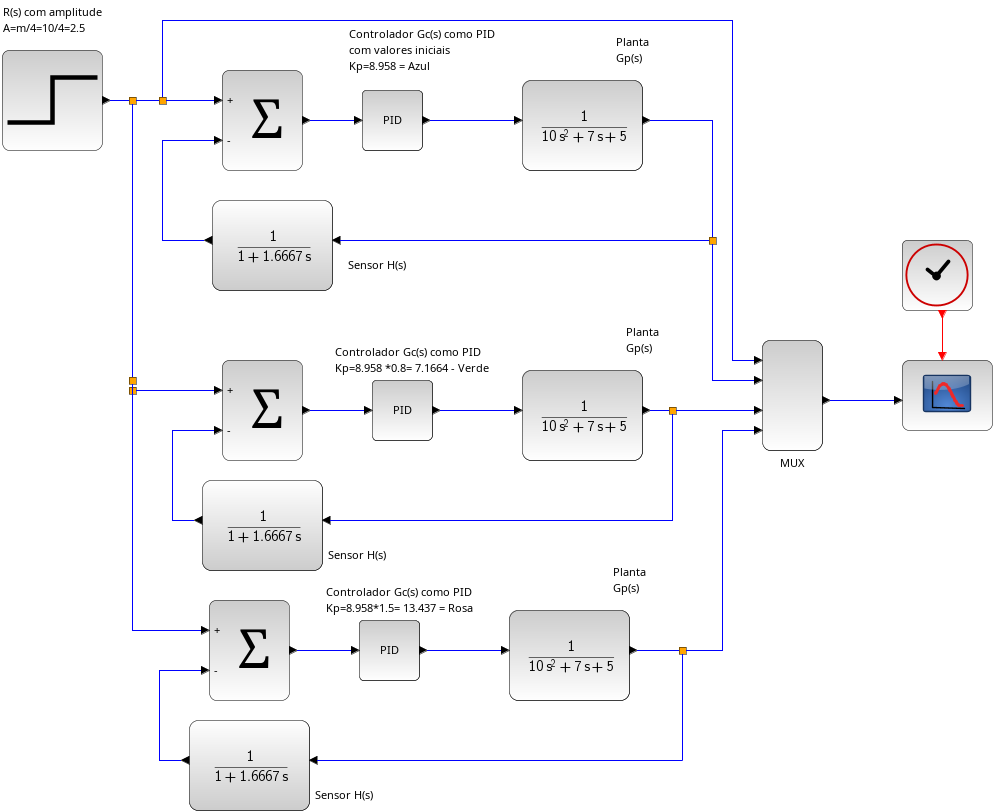
\includegraphics[width=0.8\textwidth]{atividades/6-atividade/assets/c/diagrama-pid-ajustando-kp.png}
    \caption{Diagrama de resposta do sistema com diferentes valores de \( K_p \).}
    \label{fig:diagrama-comparacao-proporcional-pid}
\end{figure}

\begin{figure}[H]
    \centering
    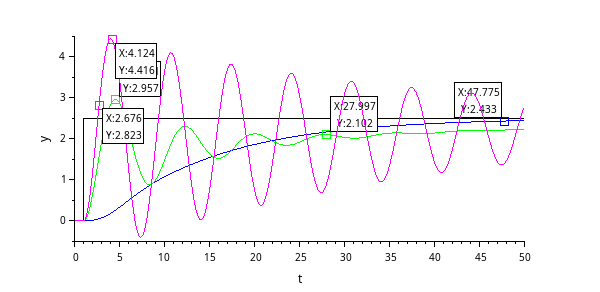
\includegraphics[width=0.8\textwidth]{atividades/6-atividade/assets/c/pid-ajustando-kp.png}
    \caption{Resposta do sistema para o \( K_p \) ajustado em comparação com outros valores.}
    \label{fig:comparacao-proporcional-pid}
\end{figure}

\subsubsection{Discussão dos Resultados e Escolha de \( K_p \)}
A análise das respostas mostrou que a redução de \( K_p \) para 7.1664 (80\% do valor inicial) oferece uma melhoria significativa em termos de controle de overshoot e estabilidade do sistema. Este ajuste resulta em uma resposta onde o overshoot é notavelmente menor, o que é vantajoso para sistemas que requerem estabilidade rápida sem oscilações excessivas.

\vspace{0.4cm}
\textbf{Vantagens:}
\begin{itemize}
    \item \textbf{Menor Overshoot:} Redução significativa no overshoot, proporcionando uma resposta mais suave e estável. Essa característica é particularmente benéfica para aplicações que não podem tolerar grandes desvios temporários de suas variáveis de processo.
    \item \textbf{Tempo de Acomodação Razoável:} O sistema atinge o estado estacionário mais rapidamente, o que é crucial para aplicações que demandam respostas rápidas e precisas. Isso é conseguido sem induzir instabilidade prolongada.
\end{itemize}

\vspace{0.4cm}
\textbf{Desvantagens:}
\begin{itemize}
    \item \textbf{Comprometimento da Rapidez Inicial:} A resposta inicial é ligeiramente mais lenta, o que pode não ser ideal para todos os tipos de aplicações, especialmente aquelas que dependem de uma atuação rápida após uma mudança de condições.
    \item \textbf{Sensibilidade a Distúrbios:} A redução do \( K_p \) pode diminuir a capacidade do sistema de reagir eficientemente a perturbações súbitas ou variações significativas na entrada, podendo resultar em um desempenho subótimo sob condições de carga variável.
\end{itemize}

Foi analisado da possibilidade de redução adicional de \( K_p \) diminuir ainda mais \( K_p \) além de 80\% poderia potencialmente levar a uma resposta demasiadamente lenta, comprometendo a capacidade do sistema de reagir a alterações rápidas. Essa mudança requer uma análise cuidadosa das prioridades do sistema: estabilidade versus rapidez de resposta.

\subsubsection{Implementação e Avaliação Futura do Novo \( K_p \)}
O novo \( K_p \) de 7.1664 será implementado no controlador PID para uso continuado. Este ajuste será acompanhado de monitoramento e avaliação contínuos para assegurar que ele atende às exigências do sistema em variadas condições operacionais.

A decisão de ajustar o \( K_p \) para 7.1664 reflete um compromisso bem fundamentado entre resposta rápida e controle de oscilações, adequado para muitas aplicações industriais e de automação. Avaliações futuras focarão em refinamentos adicionais e na otimização de \( K_i \) e \( K_d \) para maximizar a eficácia do sistema de controle.


% ===============================================================
% Letra D Validado ==============================================
\subsection{Comparação entre Controlador Proporcional, PID com Dados Iniciais e PID Ajustado}
Esta seção apresenta uma análise comparativa do desempenho de três configurações distintas de controladores: Proporcional, PID com valores iniciais e PID ajustado. A análise foca na resposta dos controladores em termos de estabilidade, tempo de resposta e precisão no estado estacionário. Ajustar o parâmetro \(K_p\) tem implicações significativas na dinâmica de controle, impactando diretamente a eficácia e eficiência do sistema.

\begin{figure}[H]
    \centering
    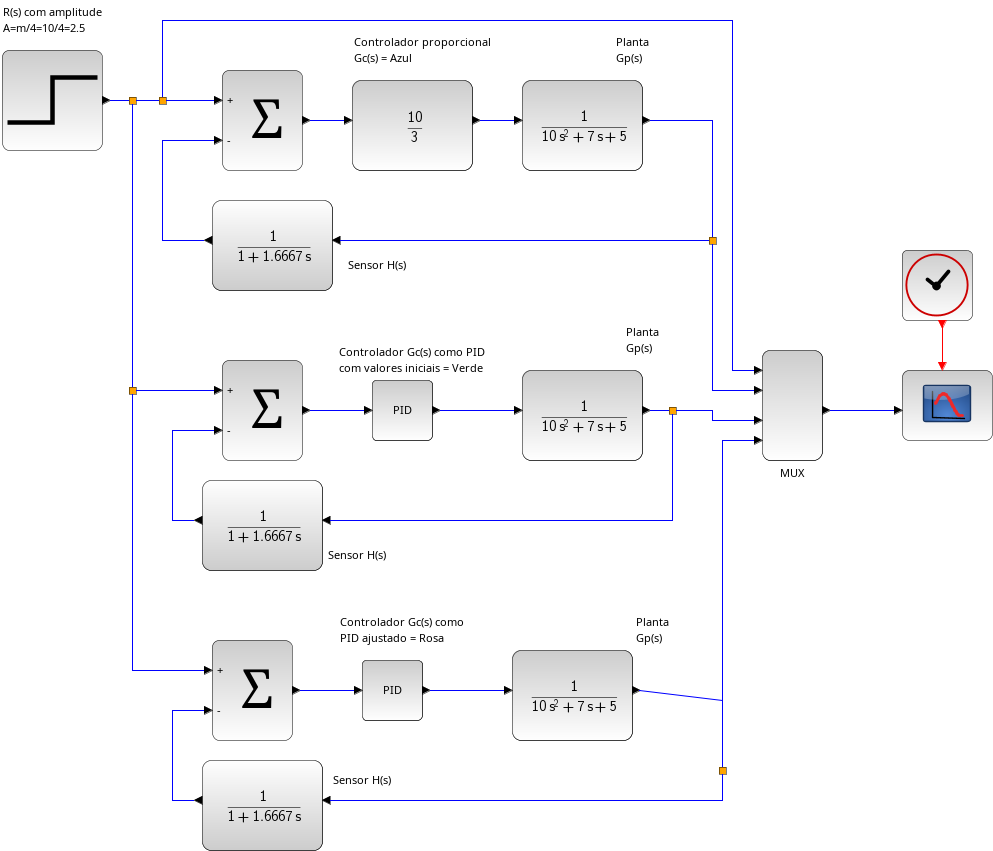
\includegraphics[width=0.8\textwidth]{atividades/6-atividade/assets/d/diagrama-comparacao-proporcional-pid-pid-ajustado.png}
    \caption{Diagrama de resposta do sistema com diferentes configurações de \(K_p\).}
    \label{fig:diagrama-comparacao-proporcional-pid-pid-ajustado}
\end{figure}

\begin{figure}[H]
    \centering
    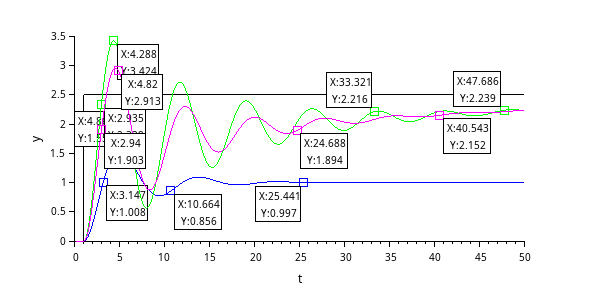
\includegraphics[width=0.8\textwidth]{atividades/6-atividade/assets/d/comparacao-proporcional-pid-pid-ajustado.png}
    \caption{Comparação das respostas temporais dos controladores sob a mesma condição de teste.}
    \label{fig:comparacao-proporcional-pid-pid-ajustado}
\end{figure}


\subsubsection{Análise dos Controladores}

\subsubsection{Controlador Proporcional (Cor Azul)}
\textbf{Comportamento:} O controlador proporcional, adequado para sistemas onde precisão extrema não é primordial, mostra uma resposta rápida inicial, mas falha em eliminar o erro de estado estacionário, uma limitação comum devido à ausência de ação integral.
\textbf{Estado Estacionário:} A resposta estabiliza significativamente abaixo do valor de referência, evidenciando a limitação deste tipo de controlador em corrigir completamente o erro de estado estacionário, adequado para aplicações onde desvios menores são toleráveis.

\subsubsection{PID com Valores Iniciais (Cor Verde)}
\textbf{Comportamento:} Este controlador exibe um overshoot inicial significativo e oscilações antes de estabilizar, característica de uma resposta rápida seguida de uma correção intensa pela ação integral.
\textbf{Estado Estacionário:} Atinge e mantém o valor desejado, com a componente integral ajustando o erro acumulado e garantindo que a saída final corresponda exatamente ao valor de referência.

\subsubsection{PID Ajustado (Cor Rosa)}
\textbf{Comportamento:} A redução de \(K_p\) para 7.1664 atenuou o overshoot e proporcionou uma abordagem mais suave na resposta ao degrau, indicando um melhor equilíbrio entre as ações proporcional e integral.
\textbf{Estado Estacionário:} Alcança o estado estacionário com menos oscilações, refletindo uma melhoria na estabilidade geral do sistema. A ação integral continua a compensar qualquer erro residual, assegurando que a saída esteja alinhada ao valor do degrau.

\subsubsection{Conclusão e Implicações para o Ajuste de \(K_p\)}
A redução de \(K_p\) para 80\% do valor inicial demonstrou melhorar a resposta do sistema ao reduzir o overshoot e aumentar a estabilidade sem comprometer excessivamente a resposta rápida. Essa modificação evidencia a necessidade de um equilíbrio cuidadoso na configuração de \(K_p\), onde a eficiência operacional e a estabilidade precisam ser otimizadas em conjunto.

\vspace{0.4cm}
\textbf{Considerações Adicionais:}
\begin{itemize}
    \item Uma redução adicional de \(K_p\) pode ser explorada para sistemas onde a estabilidade é mais crítica que a resposta rápida. No entanto, é essencial garantir que essa redução não comprometa a capacidade do sistema de responder a perturbações repentinas.
    \item O ajuste fino de \(K_p\) deve ser realizado com consideração das características específicas do sistema e das condições operacionais. A simulação controlada é recomendada para determinar o melhor conjunto de parâmetros, equilibrando estabilidade e precisão.
\end{itemize}

Embora a configuração atual de \(K_p\) tenha mostrado resultados promissores, é fundamental reconhecer que sempre existem oportunidades para refinar ainda mais os parâmetros do controlador PID. O processo de ajuste manual de \(K_p\), \(K_i\), e \(K_d\) deve ser contínuo e iterativo, adaptando-se às mudanças nas condições operacionais e às necessidades específicas de cada sistema. Ajustes manuais são essenciais para calibrar o controlador de modo a responder adequadamente sob diferentes cenários, permitindo uma melhoria contínua do desempenho do sistema.
